



	%\section{概率的朴素定义}
		\title[概率论]{第三讲:古典概型与几何概型}
	%\author[张鑫 {\rm Email: xzhangseu@seu.edu.cn} ]{\large 张 鑫}
	\institute[东南大学数学学院]{\large \textrm{Email: xzhangseu@seu.edu.cn} \\ \quad  \\
		\large 东南大学 \quad 数学学院 \\
		\vspace{0.3cm}
		% \trc{公共邮箱: \textrm{zy.prob@qq.com}\\
			% \hspace{-1.7cm}  密 \qquad 码: \textrm{seu!prob}}
	}
	\date{}


	{ \setbeamertemplate{footline}{}
		\begin{frame}
			\titlepage
		\end{frame}
	}

\subsection{古典概型}
	\begin{frame}
		\frametitle{古典概型}
		\begin{defi}(\tc{ 古典概型:}) 有两个条件,
			\begin{enumerate}[<+-|alert@+>][(1)]
				\item  (有限性) 试验结果只有有限个 (记为 $n$);
				\item (等可能性) 每个基本事件发生的可能性相同.
			\end{enumerate}

		\end{defi}

		\pause 对于古典概型: $\Omega=\{\omega_1,\cdots,\omega_n\}, \mathcal{F}=\{A:A\subset \Omega\}$, 事件 $A\in\mathcal{F}$ 的概率定义为
		\begin{eqnarray*}
			P(A)=\dfrac{|A|}{|\Omega|}, \ \forall A\in \mathcal{F}
		\end{eqnarray*}
		其中,$|B|$ 表示事件 $B$ 所包含的基本事件的个数.

	\end{frame}

\begin{frame}{古典概型的两个重要方面}
	\begin{itemize}[<+-|alert@+>]
		\item 确定样本空间与样本点\pause
		\begin{exam} 掷两个均匀硬币,出现正、反两面的概率是多少?
		\end{exam}
		\pause
		\begin{itemize}[<+-|alert@+>]
			\item 数学家d'Alembert(达朗贝尔)认为掷两个均匀硬币, 出现的结果无外乎"正正","反反","正反", %即$\Omega=\{\text{正正},\text{正反}, \text{反反}\}$,
			因此概率应是$\dfrac{1}{3}$;
			\item 事实上, 该试验样本空间为 $$\Omega=\{(\text{正, 正}),(\text{正, 反}), (\text{反, 正}), (\text{反, 反})\}$$
			\item 若硬币不可区分,则样本空间为 $\Omega=\{\{\text{正,正}\},\{\text{正,反}\}, \{\text{反,反}\}\}$, 但样本空间中的样本点并不是等可能出现, 所以也不能说出现正、反两面的概率是$\frac{1}{3}$.
		\end{itemize}
        \begin{exam}(\tc{Leibnitz的错误}) 掷两个均匀骰子,得到点数和为11与12的概率相同吗?
		\end{exam}

		\item 如何计数: 见下面计数原理.
	\end{itemize}


\end{frame}






	\begin{frame}
		\frametitle{计数原理}
			\tc{加法原理:} 考虑试验 $A$ 和 $B$, 若试验 $A$ 有 $a$ 种可能结果,试验 $B$ 有 $b$ 种可能结果,则试验 $A$ 或 $B$ 共有 $a+b$ 种结果 % 假设进行过程 $I$ 有 $n_1$ 种方式,进行过程 $II$ 均有 $n_2$ 种方式。那么,进行过程 $I$ 或 $II$ 共有 $n_1+n_2$ 种方式.
				\\
			\vspace{0.5cm}
			\pause
		\tc{乘法原理 \footnote{通常很容易想当然地认为试验是有先后顺序的,但是乘法原理并没有要求试验 $A$ 必须在试验 $B$ 之前实施。}:}   考虑一个复合试验,它由两个子试验 $A$ 和 $B$ 构成。假设试验 $A$ 有 $a$  种可能结
		果,每一种情况又都对应于试验 $B$ 的 $b$ 种可能结果。那么这个复合试验共有 $ab$ 种可能结果。% 假设进行过程 $I$ 有 $n_1$ 种方式,而对于过程 $I$ 的每一个方式,进行过程 $II$ 均有 $n_2$ 种方式。那么,依次进行过程 $I$ 与 $II$ 共有 $n_1n_2$ 种方式.\\

	\end{frame}

\begin{frame}{冰淇淋甜筒购方案计数}
	\begin{exam}
		(冰淇淋甜筒) 假没某人正在购买一支冰淇淋甜筒,甜筒有蛋卷或华夫饼两种选择,冰淇淋有巧克力 (C)、草莓 (S) 和香草 (V) 三种口味可选。考虑以下问题:
		\begin{itemize}[<+-|alert@+>]
			\item  该随机试验共有 6 种可能购买方案:无论是先决定甜简类型还是冰淇淋口味类型,试验都是总共有 $2\times 3=3\times 2=6$ 种可能
			\item  假设怀特先生某天上下午各买一支冰淇淋甜筒,则该试验共有 $6^2=36$ 种可能结果
			\item  如果只关注这天吃了何种类型的冰淇淋,而不在乎吃冰淇淋的顺序,即 $(cakeC, waffleV)$ 和 $(waffleV, cakeC)$ 之间没有区别, 则共有 \pause
			\[6*5/2+6=21\]
		 \end{itemize}
	\end{exam}


\end{frame}

\subsection{排列组合计数}


\begin{frame}
	\frametitle{排列组合}
	\begin{itemize}[<+-|alert@+>]
		\item 从 $n$ 个不同的元素中,有放回的取出 $r$ 个元素组成的排列种数为 \tc{$n^r$} 种;
		\item 从 $n$ 个不同的元素中,不放回的取出 $r$ 个元素组成的排列种数为 \tc{$$P_n^r=n (n-1)\cdots (n-r+1);$$}
		\item 从 $n$ 个不同的元素中,不放回的取出 $r$ 个元素组成的组合,种数为 \tc{$$C_n^r=\dfrac{n (n-1)\cdots (n-r+1)}{r!}=\dfrac{n!}{r!(n-r)!};$$}
		\item 从 $n$ 个不同的元素中,有放回的取出 $r$ 个元素组成的组合,种数为 \footnote{又称 Bose-Einstein 值,物理学家玻色和爱因斯坦 1920 年做了不可区分粒子的相关研究,成功预测了玻色 - 爱因斯坦凝聚态陌生物质状态的存在}
		\tc{$$C_{n+r-1}^r. $$}
	\end{itemize}
\end{frame}

	\begin{frame}
		\frametitle{生日问题}
	  \begin{exam}
	若屋子里有 $k$ 个人,假设每个人的生日都等可能为一年 365 天中的一天 (不考虑 2 月 29 日的情况),而且每个人的生日是相互独立的 (假设这里不存在双胞胎)。试问:屋内有两个及以上的人在同一天过生日的概率是多少?
	  \end{exam}
  	\pause

  	\jieda  $k$ 个人中没有人生日相同的概率为
  	\[P (\mbox{没有人生日相同})=\dfrac{365\cdot364\cdots (365-k+1)}{365^k}\]
	\pause
	故至少有两个人生日相同的概率为
\[P (\mbox{至少有两个人生日相同})=1-\dfrac{365\cdot364\cdots (365-k+1)}{365^k}\]
\pause
可以绘制至少两个人生日相同的概率随 $k$ 变化的函数图。概率首次超过 $0.5$ 是在 $k=23$, 当 $k=57$ 时,这个概率超过了 99\%.
	\end{frame}



	\begin{frame}
		\begin{exam}
			甲乙丙丁四人进行乒乓球双打练习,两人一对地结为对打的双方,有多少种不同的结对方式?
		\end{exam}\\
		\jieda 简单的组合问题:从四人中选出两人结为一对,剩下的两人结为一对即可。于是可得:
		\\
		\begin{center}
			有 $C_4^2 = 6$ 种方式. ????
		\end{center}
		\pause 但事实是否如此呢?注意此时并不要求两队之间的顺序,所以
		\begin{center}
			只有 $3$ 种结对方式: $C_4^2/2 = 3$.
		\end{center}
		\end{frame}
	\begin{frame}
		\begin{rmk}
			\begin{itemize}[<+-|alert@+>]
				\item  在按组合模式分出的 ``组内", 元素之间是没有 ``顺序" 的;
				\item 但是需要指出的是:在 ``组" 之间却存在着 ``顺序", 或者叫做 ``编号"!
				\item 在按 ``组合" 模式计算时,我们计算的是 ``取出两个人" 的所有不同取法数目.
				\item 假如我们把取出的两人算一组,而把留下的两人算另一组,那么由于 ``取出甲乙,留下丙丁" 和 ``取出丙丁,留下甲乙" 是两种不同的取出方式,而在这种计算方法中,被算作两种不同的 ``分组" 方式,从而得到 6 种 ``分组" 方式.
				\item \tc{“组合” 是一种 “有编号的分组模式”, 或者说,按照组合模式计算出的分组方式数目中,已经天然地把组的不同编号方式数目计算在内了.}

			\end{itemize}
		\end{rmk}

	\end{frame}


	\begin{frame}
		\begin{exam}
			欲将 6 个人分为 3 组,每组 2 人,分别从事 3 项不同工作,求分配方式数.
		\end{exam}\\
		\pause
		\jieda 先取出两人从事第 1 项工作,有 $C_6^2$ 种方式;再取出两人从事第 2 项工作,有 $C_4^2$ 种方式;剩下的两人从事第 3 项工作。所以一共有:\pause
		\begin{eqnarray*}
			C_6^2\cdot C_4^2= \dfrac{6!}{4!\cdot 2!}\dfrac{4!}{2!\cdot 2!}  = \dfrac{6!}{2! · 2! · 2!}=90
		\end{eqnarray*}
		种分配方式.
	\end{frame}


	\begin{frame}
		\begin{exam}
			要把 7 人分为 3 个小组,执行同一种任务,其中一个组 3 人,另两个组各 2 人,求分组方式数.
		\end{exam}\\

		\pause
		\jieda 显然这也是一个 “无编号分组” 问题。但是却与上面的情况有所不同。因为其中有一个 3 人组,无论是否编号,它都与其余两个组有所区别 (编号无非是为了对分出的组加以区分), 所以在按 “有编号分组模式” 算出分组方式数之后,只应再除以 2! (即除去两个不加区分的组的排列顺序数), \pause 故得:共有
		\begin{eqnarray*}
			\dfrac{7!}{3!\cdot 2! \cdot 2!}\cdot \dfrac{1}{2!}=\dfrac{7!}{ 3! \cdot (2!)^3}
		\end{eqnarray*}
		种分组方式.
		为了适应这种分为多个 “不同的” 组的问题需求,人们总结出如
		下的 “多组组合模式”:
	\end{frame}

	\begin{frame}
		\frametitle{多组组合与排列模式}

		\begin{itemize}[<+-|alert@+>]
			\item \tc{多组组合模式:} 有 $n$ 个不同元素,要把它们分为 $k$ 个不同的组,使得各组依次有 $n_1, n_2,\cdots, n_k$ 个元素,其中 $n_1+n_2+\cdots+n_k = n$, 则一共有
			\begin{eqnarray*}
				\dfrac{n!}{n_1! \cdot  n_2! \cdot ... \cdot  n_k!}
			\end{eqnarray*}
			种不同分法.

			\item \tc{不尽相异元素的排列模式:} 有 $n$ 个元素,属于 $k$ 个不同的类,同类元素之间不可辨认,各类元素分别有 $n_1, n_2, \cdots, n_k$ 个,其中 $n_1 +n_2 +\cdots+n_k = n$, 要把它们排成一列,则一共有
			\begin{eqnarray*}
				\dfrac{n!}{n_1! \cdot  n_2! \cdot ... \cdot  n_k!}
			\end{eqnarray*} 种不同排法.
		\end{itemize}
	\end{frame}


	\begin{frame}
		\begin{exam}
			一批产品有 $N$ 个,其中废品有 $M$ 个。现从中随机取出 $n$ 个,在以下两种情形下,分别求 “其中恰好有 $m$ 个废品” 这一事件的概率。(1) 有放回地选取;(2) 不放回地选取.
		\end{exam}
		\\
		\pause \jieda 记 $A = \{\mbox{其中恰好有} m \mbox{个废品}\}$, 则
		\begin{itemize}[<+-|alert@+>]
			\item  有放回情形: $|\Omega| = N^n, |A| = C_n^mM^m (N − M)^{n−m}$, 所以
			\begin{eqnarray*}
				P(A)=\dfrac{C_n^mM^m(N − M)^{n−m}}{N^n}=C_n^m\big(\dfrac{M}{N}\big)^m\big(\dfrac{N-M}{N}\big)^{n-m}
			\end{eqnarray*}
			\item 不放回情形: $|\Omega|=C_N^n, |A|=C_M^mC_{N-M}^{n−m}$ , 所以
			\begin{eqnarray*}
				P(A)=\dfrac{C_M^mC_{N-M}^{n−m}}{C_N^n}
			\end{eqnarray*}


		\end{itemize}

	\end{frame}
	% \begin{frame}
		%   \begin{exam}
			%     \  $n$ 个男生,$m$ 个女生排成一排 ($m≤n+1$). 求事件 $A= \{\mbox{任意两个女孩不相邻}\}$ 的概率。又若排成一圈,又如何?
			%   \end{exam}
		%   \\ \pause \jieda
		%   \begin{itemize}[<+-|alert@+>]
			%   \item 排成一排:
			%     \begin{eqnarray*}
				%       |\Omega| &=& (n+m)!,\quad     |A| = n!C_{n+1}^m m!,\\
				%       P(A)&=&\dfrac{|A|}{|\Omega|}=\dfrac{n!C_{n+1}^m m!}{(n + m)!}
				%     \end{eqnarray*}
			%   \item 排成一圈:
			%     \begin{eqnarray*}
				%       |\Omega| &=& (n+m-1)!,\quad     |A| = (n-1)!C_{n}^m m!,\\
				%       P(A)&=&\dfrac{|A|}{|\Omega|}=\dfrac{(n-1)!C_{n}^m m!}{(n + m-1)!}
				%     \end{eqnarray*}

			%   \end{itemize}
		% \end{frame}

%	\begin{frame}
%	  \begin{exam}
%		    \ $r$ 个不同的球任意放入编号为 $1$ 至 $n$ 的 $n$ 个盒子,每球入各盒均等可能,求下列事件的概率:
%		    \begin{itemize}
%			    \item[(1)]  $A=\{\mbox{指定的} r \mbox{个盒子各含一个球}\}$,
%			    \item[(2)] $B=\{\mbox{每盒至多有一球}\}$,
%			    \item[(3)]  $C=\{\mbox{某指定盒中恰有} m \mbox{个球}\}$.
%			    \end{itemize}
%		  \end{exam}
%	  \pause  \jieda  $|\Omega|=n^r$
%	  \begin{itemize}[<+-|alert@+>]
%		  \item[(1)] $|A|=r!$, $P(A)=\dfrac{r!}{n^r}$;
%		  \item[(2)] $|B|=C_n^r r!$, $P(B)=\dfrac{C_n^rr!}{n^r}$;
%		  \item[(3)] $|C|=C_r^m(n-1)^{r-m}$, $P(C)=\dfrac{C_r^m(n-1)^{r-m}}{n^r}$
%		  \end{itemize}
%	\end{frame}

%	 \begin{frame}
%		   \vspace{0.3cm}
%		   \begin{exam}
%			     \ $r$ 个相同的球任意放入编号为 $1$ 至 $n$ 的 $n$ 个盒子,每球入各盒均等可能,求下列事件的概率:
%			     \begin{itemize}
%				     \item[(1)]  $A=\{\mbox{指定的} r \mbox{个盒子各含一个球}\}$,
%				     \item[(2)] $B=\{\mbox{每盒至多有一球}\}$,
%				     \item[(3)]  $C=\{\mbox{某指定盒中恰有} m \mbox{个球}\}$.
%				     \end{itemize}
%			   \end{exam}
%
%		   \pause \jieda 我们只需要关心各个盒子中的球数,而无需考虑哪个球落在哪个盒子中。我们可把问题设想为:
%
%		   \qquad  $r$ 个相同的小球已经一字排开,只须在它们之间加上 $n − 1$ 块隔板,把它们隔为 $n$ 段,然后让各段对号放入相应的盒子即可. \pause 由于盒子可空,相当于要将 $r + n − 1$ 个不尽相异的元素进行排列,其中 $1$ 类元素 (小球) 有 $r$ 个,另 1 类元素 (隔板) 有 $n − 1$ 个,所以由不尽相同元素的排列模式知,一共有 \pause
%		   \begin{eqnarray*}
%			     \dfrac{(r+n-1)!}{r!\cdot (n-1)!}=C_{r+n-1}^{n-1}
%			   \end{eqnarray*}
%		   种不同分法. \pause 故 $|\Omega|=C_{r+n-1}^{n-1}$. 而 $|A|=1,  |B|=C_n^r, |C|=C_{r-m+n-1-1}^{r-m}$.
%		 \end{frame}
%
%	\begin{frame}
%		\begin{rmk}
%			\begin{itemize}[<+-|alert@+>]
%				\item 球相异和球相同两种情形下的样本空间是不同的,即机会均等原则是不同的。(各是什么呢?)
%
%				\item 这个例子是古典概型中一个很典型的问题,不少实际问题可以归结为它.
%
%				\item 若把球解释为粒子,把盒子解释为相空间中的小区域,则这个问题便相应于统计物理学里的 Maxwell—Boltzmann 统计.
%				\item 生日问题:求 $r$ 个人中没有两个人生日相同的概率.
%				\item 若把 $r$ 个人看作上面问题中的 $r$ 个球,而把一年的 $365$ 天看作为盒子,则 $n = 365$, 这时事件 $B$ 的概率即为所求概率.
%				\item 例如当 $r = 40$ 时,$P (B) = 0.109$, 这个概率已经相当小;而当 $r = 50$ 时,$P (B) = 0.03$. 进一步当 $r = 55$ 时,$P (B)$ 之值只有 $0.01$, 这实在是出乎意料地小.
%
%			\end{itemize}
%		\end{rmk}
%	\end{frame}
%
%






	\begin{frame}%{古典概型的实例}
		\begin{exam}
			\label{exam1.2}
			一个笼子里关着 7 只白猫和 3 只黑猫共 10 只猫,把笼门打开每次只允许钻出 1 只猫。若 10 只猫均钻出笼子,并以 $A_k$ 表示事件 ``第 $k$ 只出笼的猫是黑猫",试求 $P (A_k)$,其中,$k=1,2,...,10$.
		\end{exam}


	\end{frame}
	\begin{frame}
		\textcolor{cyan}{方法一}:将 10 只猫看成不同的猫
		\begin{itemize}[<+-|alert@+>]
			\item  $|\Omega|=10!$
			\item  $\left|A_{k}\right|=C_3^1 \cdot 9!$
			\item $
			P\left(A_{k}\right)=\dfrac{\left|A_{k}\right|}{|\Omega|}=\dfrac{3 \cdot 9 !}{10 !}=\dfrac{3}{10}, \quad k=1,2, \cdots, 10 .	$
		\end{itemize}



	\end{frame}


	\begin{frame}%{例 \ref{exam1.2} 的另外一种解法}
		\textcolor{cyan}{方法二}:仅白猫与黑猫可区别
		\begin{itemize}[<+-|alert@+>]
			\item 现在只有两种不同的元素,一种有 7 个 (7 只白猫), 另一种有 3 个 (3 只黑猫), 由不尽相异元素的排列模式知
			$$|\Omega|=C_{10}^3=120$$
			\item  $\left|A_{k}\right|=C_9^2=36$

			\item $
			P\left(A_{k}\right)=\frac{36}{120}=\frac{3}{10}, \quad k=1,2, \cdots, 10 .
			$
		\end{itemize}

	\end{frame}
	\begin{frame}%{例 \ref{exam1.2} 的第三种解法}
		\textcolor{cyan}{方法三}:仅考虑前 $k$ 只出笼猫的排列情况 % 白猫与黑猫可区别
		\begin{itemize}[<+-|alert@+>]
			\item $|\Omega|=C_{10}^k\cdot k!=\dfrac{10!}{(10-k) !}$
			\item $\left|A_{k}\right|=C_{3}^1\cdot C_{9}^{k-1}\cdot (k-1)!=\dfrac{3 \cdot 9!}{(10-k) !}$
			\item  $
			P\left(A_{k}\right)=\dfrac{3 \cdot 9 !}{10 !}=\dfrac{3}{10}, \quad k=1,2, \cdots, 10
			$
		\end{itemize}

		%	\begin{rmk}
			%		\begin{itemize}
				%			\item 概率计算问题不同于普通的计数问题;
				%			\item 在概率计算问题中,保证对两者采用同一种计数模式
				%		\end{itemize}
			%	\end{rmk}
	\end{frame}

	% \begin{frame}
		%   \begin{exam}
			%     设有方程 $x + y + z = 15$, 试分别求出它的正整数解和非负整数解 $(x,y,z)$ 的组数.
			%   \end{exam}
		%   \\
		%   \pause \jieda 本题可以设想为将 $ 15 $ 个无区别的小球分入 $ 3 $ 个不同的盒子,再分别将第 $ 1, 2, 3 $ 个盒中的球数对应为 $ x, y, z $ 的值即可。所以,非负整数解的组数 (相当于允许出现空盒的情况) 为:\pause
		%   \begin{eqnarray*}
			%     C_{15+3-1}^{15}=C_{17}^2=\dfrac{17\times 16}{2}=136
			%   \end{eqnarray*}
		%   \pause 而正整数解的组数 (相当于不允许出现空盒的情况) 为:
		%   \begin{eqnarray*}
			%     C_{15-1}^{3-1}=C_{14}^2=\dfrac{14\times 13}{2}=91
			%   \end{eqnarray*}

		% \end{frame}

	% \begin{frame}
		%   \frametitle{思考}
		%   设有 $n$ 个人随机地坐到礼堂第一排 $N$ 个座位上去,试求下列事 件的概率:(1) 任何人都没有邻座;(2) 每人恰有一个邻座;(3) 关于中央座位对称的两个座位至少有一个空着。

		% \end{frame}
\begin{frame}{``球-盒"计数问题}
	\begin{itemize}
		\item $S(n,k)$:第二类Stirling数, 表示将$n$个元素的集合分解为$k$个非空子集的分法数目;
		%\item 例如,${S(3,2)=3}$,即 3 个元素的集合${\{1,2,3\}}$可以分为
		%\[{\{1,2\} \cup\{3\},\{1,3\} \cup\{2\},\{3,2\} \cup\{1\}}.\]
		\item 不难验证$S(n+1, k)=k S(n, k)+S(n, k-1)$, 并可以证明(枚举空盒的个数,剩下的随便放,盒子是相同的最后要除以$m!$)
		\[
		S(n, k)=\frac{1}{k!} \sum_{j=0}^{k}(-1)^{j}C_k^j (k-j)^{n}
		\]
		\item ${p(n, k)}$: 表示将${n}$分解为${k}$个正整数之和的分法数目. ${(p(n, k)}$的计算相当复杂, 涉及整数以及集合分拆的问题, 有兴趣的可参阅组合计数方面的文献).
	\end{itemize}
\pause
	\begin{table}[]
		\begin{tabular}{|c|cc|cc|}
		\hline
		\rowcolor[HTML]{CBCEFB}
		\cellcolor[HTML]{CBCEFB}{\color[HTML]{000000} }                                                                         & \multicolumn{2}{c|}{\cellcolor[HTML]{CBCEFB}{\color[HTML]{000000} 盒可区分}}                                & \multicolumn{2}{c|}{\cellcolor[HTML]{CBCEFB}{\color[HTML]{000000} 盒不可区分}}                               \\ \cline{2-5}
		\rowcolor[HTML]{CBCEFB}
		\multirow{-2}{*}{\cellcolor[HTML]{CBCEFB}{\color[HTML]{000000} \begin{tabular}[c]{@{}c@{}}$n$个球\\ $r$个盒子\end{tabular}}} & \multicolumn{1}{c|}{\cellcolor[HTML]{CBCEFB}{\color[HTML]{000000} 允许空盒}} & {\color[HTML]{000000} \begin{tabular}[c]{@{}c@{}}不允许空盒\\ $n>r$\end{tabular}} & \multicolumn{1}{c|}{\cellcolor[HTML]{CBCEFB}{\color[HTML]{000000} 允许空盒}} & {\color[HTML]{000000} \begin{tabular}[c]{@{}c@{}}不允许空盒\\ $n>r$\end{tabular}} \\ \hline
		\rowcolor[HTML]{ECF4FF}
		\cellcolor[HTML]{CBCEFB}{\color[HTML]{000000} 球可区分}                                                                     & \multicolumn{1}{c|}{\cellcolor[HTML]{ECF4FF}{\color[HTML]{000000} $r^n$}}    & {\color[HTML]{000000} $r!S(n,r)$}     & \multicolumn{1}{c|}{\cellcolor[HTML]{ECF4FF}{\color[HTML]{000000} $\sum_{k=1}^rS(n,k)$}}    & {\color[HTML]{000000} $S(n,r)$}     \\ \hline
		\rowcolor[HTML]{ECF4FF}
		\cellcolor[HTML]{CBCEFB}{\color[HTML]{000000} 球不可区分}                                                                    & \multicolumn{1}{c|}{\cellcolor[HTML]{ECF4FF}{\color[HTML]{000000} $C_{n+r-1}^n$}}    & {\color[HTML]{000000} $C_{(n-r)+r-1}^{n-r}$}     & \multicolumn{1}{c|}{\cellcolor[HTML]{ECF4FF}{\color[HTML]{000000} $\sum_{k=1}^rp(n,r)$}}    & {\color[HTML]{000000} $p(n,r)$}     \\ \hline
		\end{tabular}
		\end{table}
\end{frame}
\subsection{统计物理模型}
\begin{frame}{{\rm Maxwell-Boltzmann}(麦克斯韦-玻尔兹曼)统计}
\begin{itemize}[<+-|alert@+>]
	\item 考查热平衡系统以及其中的粒子,在温度充分高且分布的密度足够低,粒子间的量子效应可以忽略.
	\item 假定能态被标记为${\{1,2,\cdots,K\}}$,粒子的总数为${N}$,那么恰有${N_{i}}$个粒子处于能态${i}$上的概率为
	\[P_{\mathrm{M}-\mathrm{B}}=K^{-N}\frac{N!}{N_{1}!N_{2}!\cdots N_{K}!},\quad N_1+\cdots+N_K=N.\]
	\item Maxwell-Boltzmann 统计最重要的假设是粒子的可区分性.
	\item 该假设条件下粒子 A 处于能态 1 且粒子 B 处于能态 2 , 与粒子 A 处于能态 2 且粒子 B 处于能态 1 是不同的两种系统状态.
	\item 该假设所导出的粒子的能态分布 (即 Boltzmann 分布) 较为符合物理事实.
	\item 但是其在熵方面却导致了和物理事实严重违背的结果 (所谓的 Gibbs 悖论), 而一旦假设粒子不可区分, 则矛盾会迎刃而解.
\end{itemize}



\end{frame}


\begin{frame}{{\rm Bose-Einstein}(博兹-爱因斯坦)统计}
\begin{itemize}[<+-|alert@+>]
	\item 当温度下降, 且粒子的空间密度上升时, 粒子间的量子效应变得显著而不可忽略, 粒子在能态间的分布也随之发生变化.
	\item 根据表现的不同, 可将粒子分为两类:玻色子 (Boson) 和费米子 (Fermion).
	\item 无穷多个玻色子能够在同一时间处于("凝聚") 同一能态上, 从而出现统计物理学中著名的 Bose-Einstein 凝聚 (Bose-Einstein condensate) 现象.
	\item 假定粒子总数为 \( N \)但粒子不可区分, 能态数目为 \( K \), 则玻骰子在各能态上的分布服从 Bose-Einstein 统计,
	\[
	P_{\mathrm{B}-\mathrm{E}}%=\frac{1}{B_{N}^{K}}
	=\dfrac{1}{C_{N+K-1}^N}=\binom{N+K-1}{N}^{-1}
	\]
	\item Bose-Einstein 统计的粒子能态分布情况与 \( N \) 个不可区分的球放入 \( K \) 个可区分的盒中的放法形成一一对应.
\end{itemize}



\end{frame}


\begin{frame}{{\rm Fermi-Dirac}(费米-狄利克雷)统计}

\begin{itemize}[<+-|alert@+>]
	\item 费米子遵守量子力学中的 Pauli 不相容原则,即不同的粒子无法处在相同的能态上 (注意玻色子是不满足这一原则的).
	\item 因此, 系统中的粒子数目一定比能态数目少, 即 \( N<K \).
	\item 费米子的能态服从 Fermi-Dirac 分布,
	\[
	P_{\mathrm{F}-\mathrm{D}}=\dfrac{1}{C_K^N}=\binom{K}{N}^{-1}
	\]
	\item 该分布对应于 \( N \) 个不可区分的球放入 \( K \) 个可区分的盒中, 且每个盒里不能多于两球的放法数目.
	\item Fermi-Dirac 统计在帮助人们理解电子的行为方面起到了非常关键的作用.
\end{itemize}

\end{frame}



	\subsection{几何概型}
	\begin{frame}
		\frametitle{几何概型的基本思想}
		\vspace{-0.3cm}
		\begin{enumerate}[<+-|alert@+>]
			\item 可度量性。样本空间 $\Omega$ 充满某个区域,其度量 (长度、面积、体积) 大小可用 $S_{\Omega}$ 表示;
			\item 等可能性。任意一点落在度量相等的子区域内是等可能的,即任一子区域 $A$ 的概率,只与子区域的度量 $S_A$ 有关, 而与子区域的位置无关;
			\item 若事件 $A$ 为 $\Omega$ 的某个子区域,且其度量大小可用 $S_A$ 表示,则事件 $A$ 的概率为
			\begin{eqnarray*}
				P(A)=\frac{S_A}{S_{\Omega}}
			\end{eqnarray*}
		\end{enumerate}
		\vspace{-0.5cm}
		\pause \begin{figure}%[!h]
			\centering
			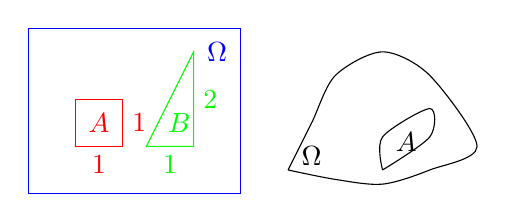
\begin{tikzpicture}[scale=0.6]
				% \begin{scope}
					%   \clip \firsrectangle;
					%   \fill[red] \secondrectangle;
					% \end{scope}
				% \begin{scope}
					%   \clip \firstcircle;
					%   \clip \secondcircle;
					%   \fill[green] \thirdcircle;
					% \end{scope}
				\draw[blue] (-0.5,-0.5) rectangle (4,3) node at (3.5,2.5){$\Omega$};
				\draw[red] (0.5,0.5) rectangle (1.5,1.5) node at (1,1){$A$};
				\draw[green] (2,0.5)--(3,0.5)--(3,2.5)--cycle node at (2.7,1) {$B$};
				\draw[red] node[below] at (1,0.5){$1$};
				\draw[green] node[below] at (2.5,0.5){$1$};
				\draw[red] node[right] at (1.5,1){$1$};
				\draw[green] node[right] at (3,1.5){$2$};

				\draw plot[smooth] coordinates %
				{(5,0) (6,-0.2) (7,-0.3) (8,0) (9,0.5) (8,2) (7,2.5) (6,2) (5.5,1) (5,0)} node at (5.5, 0.3){$\Omega$};
				\draw plot[smooth] coordinates %
				{( (7,0) (8,0.7) (8,1.3) (7,0.7) (7,0)} node at (7.5, 0.6){$A$};

				% \draw \firsttriangle node {$B$};
				% \draw \thirdcircle node {$C$};
				% \draw[rounded corners] (-2.5,-4) rectangle (4.5,2.5);
			\end{tikzpicture}
			% \caption{Till Tantau 给的一个例子 \label{tantau}}
		\end{figure}

	\end{frame}
	\begin{frame}
		\vspace{0.2cm}
		\begin{exam}\tc{ 蒲丰投针问题}: 平面上画有间隔为 $d$ 的等距平行线, 向平面任意投掷一枚长为 $l$ 的针, 求针与平行线相交的概率.
		\end{exam}
		\begin{figure}[htbp]
			\pause
			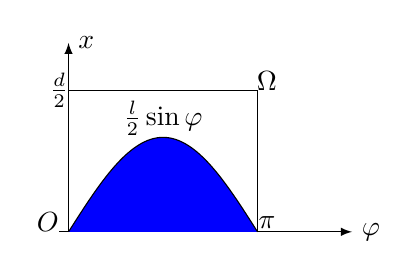
\begin{tikzpicture}[scale=1.2]
				\draw[->,>=latex] (-0.1,-2)--(3,-2) node[right]{$\varphi$};
				\draw[->,>=latex] (0,-2)--(0,0) node[right]{$x$};
				\draw node[left] at (0,-1.9){$O$};
				\draw[fill=blue] (0,-2) sin (1,-1) cos (2,-2);
				\draw (0,-0.5)--(2,-0.5)--(2,-2);
				\draw node at (-0.1,-0.5){$\frac{d}{2}$};
				\draw node at (2.1,-1.9){$\pi$};
				\draw node at (2.1,-0.4){$\Omega$};
				\draw node at (1,-0.8){$\frac{l}{2}\sin \varphi$};
			\end{tikzpicture}
			% \caption{蒲丰投针问题中的 $\Omega$ 和 $A$}
			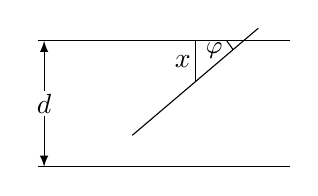
\begin{tikzpicture}[scale=0.8]
				\draw (0,0)--(4,0);
				\draw (0,-2)--(4,-2);
				\draw[->,>=latex] (0.1,-0.8)--(0.1,0);
				\draw[->,>=latex] (0.1,-1.2)--(0.1,-2);
				\draw node at (0.1,-1){$d$};
				\draw (1.5,-1.5)--(3.5,0.2);
				\draw (2.5,-0.65)--(2.5,0) node at (2.3,-0.33){$x$};
				\draw plot[smooth] coordinates%
				{(3,0) (3.1,-0.14)} node at (2.8,-0.15){\small$\varphi$};
			\end{tikzpicture}
			% \caption{蒲丰投针问题}
		\end{figure}

		\jieda 注意到 \vspace{-0.8cm}
		\begin{eqnarray*}
			\Omega&=&\{(\varphi,x):0\le x\le d/2, 0\le\varphi \le \pi\}\\
			A&=&\{\mbox{针与平行线相交}\}\\
			&=&\{(\varphi,x):x\leq \frac{l}{2}\sin\varphi\}
		\end{eqnarray*}
		由几何概型知
		\[P(A)=\frac{S_A}{S_\Omega}=\frac{\int_0^\pi\frac{l}{2}\sin\varphi d\varphi}{\frac{d}{2}\pi}=\frac{2l}{d\pi}.\]
	\end{frame}
	\begin{frame}
		\frametitle{随机模拟}
		\vspace{-0.2cm}
		\begin{itemize}
			\item $l,d$ 已知,将 $\pi$ 的值代入即可计算 $P (A)$ 的值;
			\item 若我们以频率近似概率 $P (A)$, 即
			\begin{eqnarray*}
				\frac{n}{N}\approx P(A)=\frac{2l}{d\pi}
			\end{eqnarray*}
			则我们可得到 $\pi$ 的近似值
			\begin{eqnarray*}
				\pi\approx \frac{2lN}{dn}
			\end{eqnarray*}
		\end{itemize}
		\vspace{-0.5cm}
		\pause
		\begin{table}
			\centering
			\caption{历史试验数据}
			\rowcolors[]{1}{blue!20}{blue!10}
			\begin{tabular}{|c|c|c|c|c|c|}
				\hline
				\rowcolor{blue!50}
				试验者 & 年份  &$l/d$ & 投掷次数 & 数交次数 &$\pi$ 的近似值 \\
				\hline
				Wolf & 1850 & 0.8  & 5000 &  2532 &3.1596\\
				Fox  & 1884 & 0.75  &1030 &  489  &3.1595\\
				Lazzerini & 1901 & 0.83  &3408 &  1808 &3.1415\\
				Reina & 1925 & 0.54  & 2520 &  859 &3.1795\\
				\hline
			\end{tabular}
		\end{table}
	\end{frame}
	\begin{frame}
		\frametitle{会面问题}
		\begin{exam}
			甲乙约定在下午 6 点到 7 点之间在某处会面,并约定先到者等候另一个人 20 分钟,过时即可离去,求两人能会面的概率.
		\end{exam}
		\pause
		\begin{columns}
			\hspace{-1cm}\column{6cm}
			\jieda 以 $x$ 和 $y$ 分别表示甲乙两人到达约地点的时间(以分钟为单位), 则易知:
			\begin{eqnarray*}
				\Omega&:=&\{(x,y):  0\leq x\leq 60,\quad 0\leq y\leq 60
				\}\\
				A&:=&\{(x,y):|x-y|\leq 20\}
			\end{eqnarray*}\pause
			故
			\begin{eqnarray*}
				P(A)=\frac{S_A}{S_\Omega}=\frac{60^2-40^2}{60^2}=\frac{5}{9}.
			\end{eqnarray*}
			\column{3cm}
			\begin{figure}[htbp]
				\centering
				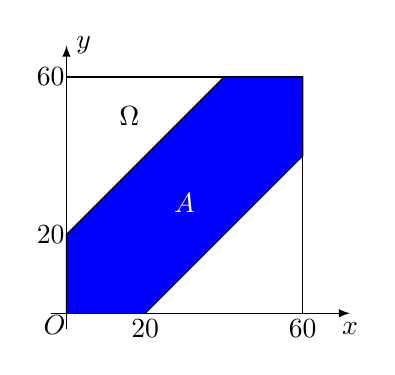
\begin{tikzpicture}
					\draw[->,>=latex] (-0.2,-3.2)--(3.6,-3.2) node[below]{$x$};
					\draw[->,>=latex] (0,-3.4)--(0,0.2) node[right]{$y$};
					\draw node at (-0.15,-3.35){$O$};
					\draw (0,-0.2)--(3,-0.2)--(3,-3.2);
					\draw[fill=blue] (0,-3.2)--(0,-2.2)--(2,-0.2)--(3,-0.2)--(3,-1.2)--(1,-3.2);
					\draw node at (-0.2,-2.2){$20$};
					\draw node at (-0.2,-0.2){$60$};
					\draw node at (0.8,-0.7){$\Omega$};
					\draw node at (1.5,-1.8){${\color{white} A}$};
					\draw node at (1,-3.4){$20$};
					\draw node at (3,-3.4){$60$};
				\end{tikzpicture}
			\end{figure}
		\end{columns}
	\end{frame}

	% \begin{frame}
		%   \vspace{0.4cm}
		%   \begin{exam}
			%     在长度为 $a$ 的线段内任取两点将其分为三段,求可以构成一个三角形的概率.
			%   \end{exam}

		%   \jieda 分别用 $x,y, a-x-y$ 表示分成的三段长度,则样本空间
		%   \begin{eqnarray*}
			%     \Omega  = \{(x,y):0<x<a,0<y<a,0<x+y<a\}
			%   \end{eqnarray*}
		%   \vspace{-0.6cm}    \begin{columns}
			%     \column{6.5cm}
			%     $x,y,a-x-y$ 成三角形 $\Leftrightarrow$
			%     \begin{eqnarray*}
				%       &&0<a-(x+y)<x+y,\\
				%       &&0<x<y+(a-x-y),\quad  \Rightarrow\\
				%       &&0<y<x+(a-x-y),
				%     \end{eqnarray*}
			%     $A=\{(x,y):0<x,y<\frac{a}{2}<x+y<a\}$. 从而 $$P (A)=\frac{S_A}{S_\Omega}=1/4.$$
			%     \column{4cm}
			%     \vspace{-0.5cm}
			%     \begin{figure}[htbp]
				%       \centering
				%       \begin{tikzpicture}
					%         \draw[|-|] (0,0)--(1,0);
					%         \draw[-|] (1,0)--(2.3,0);
					%         \draw[-|] (2.3,0)--(4,0);
					%         \draw[|-,style=dashed] (0,-0.4)--(1.9,-0.4);
					%         \draw[-|,style=dashed] (2.1,-0.4)--(4,-0.4);
					%         \draw node at  (0.5,0.2){$x$};
					%         \draw node at  (1.65,0.2){$y$};
					%         \draw node at  (3.15,0.2){$a-x-y$};
					%         \draw node at  (2,-0.4){$a$};
					%       \end{tikzpicture}
				%     \end{figure}
			%     \vspace{-1.8cm}
			%     \begin{figure}[htbp]
				%       \centering
				%       \begin{tikzpicture}
					%         \draw[->,>=latex] (-0.2,-3.2)--(3.6,-3.2) node[below]{$x$};
					%         \draw[->,>=latex] (0,-3.4)--(0,0.2) node[right]{$y$};
					%         \draw (0,-0.2)--(3,-3.2);
					%         \draw node at (-0.15,-3.35){$O$};
					%         \draw[fill=red] (0,-1.7)--(1.5,-1.7)--(1.5,-3.2)--cycle;
					%         \draw node at (-0.3,-1.7){$a/2$};
					%         \draw node at (-0.2,-0.2){$a$};
					%         \draw node at (0.5,-1){$\Omega$};
					%         \draw node at (1,-2){${\color{white} A}$};
					%         \draw node at (1.5,-3.4){$a/2$};
					%         \draw node at (3,-3.4){$a$};
					%       \end{tikzpicture} \end{figure}
			%   \end{columns}

		% \end{frame}
	\begin{frame}
		\frametitle{贝特朗奇论}
		\begin{exam} 在一圆内任取一条弦,问其长度超过该圆内接等边三角形的边长的概率是多少?
		\end{exam}
		\vspace{-0.5cm}
		\begin{columns}
			\column{3cm}
			\begin{figure}[htbp]
				\centering
				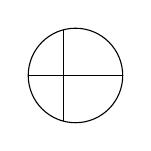
\begin{tikzpicture}[scale=0.6]
					\draw (-1,0)--(1,0);
					\draw (0,0) circle (1);
					\draw (105:1)--(255:1);
				\end{tikzpicture}
			\end{figure}
			\column{3cm}
			\begin{figure}[htbp]
				\centering
				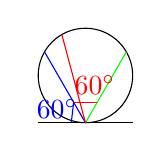
\begin{tikzpicture}[scale=0.6]
					\draw (-1,-1)--(1,-1);
					\draw (0,0) circle (1);
					\draw[blue] (0,-1)--(150:1);
					\draw[green] (0,-1)--(30:1);
					\draw[red] (0,-1)--(120:1);
					% \draw (-0.5,-1) arc (-0.25,-0.57);
					\draw[blue] plot[smooth] (-0.3,-1)--(-0.25,-0.57);
					\draw[red] plot[smooth] (-0.25,-0.57)--(0.25,-0.57);
					\node at (-0.6,-0.7){\color{blue}$60^\circ$};
					\node at (0.2,-0.2){\color{red}$60^\circ$};
				\end{tikzpicture}
			\end{figure}
			\column{3cm}
			\begin{figure}[htbp]
				\centering
				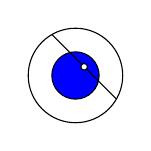
\begin{tikzpicture}[scale=0.6]
					\draw (0,0) circle (1);
					\draw[fill=blue] (0,0) circle (0.5);
					\draw (120:1)--(330:1);
					\draw[fill=white] (45:0.26) circle (2pt);
					% \coordinate (a) at (120:1);
					% \coordinate (b) at (345:1);
					% \draw[red] (a) -- (b);
					% \coordinate (c) at ($ (a)!.5:(b) $);
					% \draw[->,green] (a) -- (c);
					% \draw ((120:1)!.5:(345:1)) circle (2pt);
				\end{tikzpicture}
			\end{figure}
		\end{columns}
		{\small \jieda 易知,圆内接正三角形的边长 $\sqrt{3} R$
			\begin{enumerate}[<+-|alert@+>]
				\item 注意到弦的长度与它与圆心的距离有关,而与弦的方向无关。显然,当且仅当弦与圆心的距离小于 $R/2$ 时,弦的长超过 $\sqrt{3} R$, 故概率为 $1/2$;
				\item 把弦的一端固定,另一端点在圆周上随机移动。若在固定端点作一切线,则与切线交角在 $60^\circ$ 与 $120^\circ$ 之间的弦才能超过 $\sqrt{3} R$. 故所求概率为 $1/3$;
				\item 弦长被其中点位置决定,则当且仅当弦的中点落在半径为 $R/2$ 的小圆内时,弦的长度才会超过 $\sqrt{3} R$, 故所求概率为 $1/4$.

			\end{enumerate}
		}
	\end{frame}
%	\begin{frame}
%		\frametitle{确定概率的主观方法}
%		\vspace{-0.3cm}
%		\begin{itemize}
%			\item 统计界的贝叶斯学派认为:{\color{red} 一个事件的概率是人们根据经验对该事件发生的可能性所给出的个人信念}. 这样给出的概率称为{\color{red} 主观概率}
%			\begin{itemize}
%				\item 天气预报中,“明天下雨的概率为 $90\%$”;
%				\item 企业家根据经验及市场信息,认为 “某项新产品在未来市场上会畅销的可能性为 $80\%$”;
%			\end{itemize}
%			\pause \item 主观概率的特点
%			\begin{itemize}
%				\item 主观概率与主观臆造有本质上的不同,主观概率要求当事人对所考察的事件有透彻的了解和丰富的经验,因此主观概率是可信的;
%				\item 主观概率本质上是对随机事件概率的推断与估计,虽精确性有待检验,但结论的可信性在统计意义上是有价值的;
%				\item 随机现象无法大量重复时,用主观方法做决策和判断是适合的,可以看成频率方法的一种补充;
%				\item 主观概率除根据自已的经验外,还可以利用别人的经验.
%			\end{itemize}
%
%		\end{itemize}
%	\end{frame}

